%======================================================================
% PoznQMI-7.pdf
%======================================================================
\section{Unitární časový vývoj}
\strana{QM-T-1}

\kw{časová Schrödingerova rovnice}:
\[
  \vzorec{i\hbar\pdv{t}\ket{\psi(t)} = H\ket{\psi(t)}} \qquad (\text{tSR})
\]
\dots\ odvodili jsme pro bezstrukt.\ částici, ale \underline{POSTULUJEME OBECNĚ} \\
\hspace*{6cm} $\to$ existence $H$ pro $\forall$ systém

\underline{formální řešení:} \quad
$\ket{\psi(t-s)} = J_s\ket{\psi(t)} = e^{\frac{i}{\hbar}H\cdot s}\ket{\psi(t)}$ \\
\hspace*{6.2cm} $\uparrow$ čas.\ posun v Galilei transf.

obvyklejší zápis: \quad $\ket{\psi(t+s)} = e^{-\frac{i}{\hbar}Hs}\ket{\psi(t)} \equiv U(s)\ket{\psi(t)}$ \\
\phantom{obvyklejší zápis:} \quad nebo \quad
$\ket{\psi(t')} = U(t',t)\ket{\psi(t)} = e^{-\frac{i}{\hbar}(t'-t)H}\ket{\psi(t)}$ \\
\hspace*{3cm} \sout{OPERÁ} \kw{EVOLUČNÍ OPERÁTOR} $\nearrow$

\underline{pozn:} (tSR) lze zobecnit rovněž na interakci, tj.\ $H$ explicitně závislé na čase. Řešení (tSR) pak \pozor{NELZE} psát jako exp! \\
\quad $\to$ příští semestr \dots\ Dysonova řada jako zákl.\ poruch.\ počtu \\
\quad\quad \dots\ nebo numericky jako difro v $t$ \dots \quad
$\to\ \ket{\psi(t+\Delta t)} \simeq \ket{\psi(t)} + \frac{H}{i\hbar}\Delta t\ket{\psi(t)}$ \\
\quad NAPŘ: vnější pole $A(Q)$, $V(Q)$ záv.\ na čase

\subsection{Stac.\ stavy a int.\ pohybu}
pro čas.\ nezáv.\ $H$: \quad \dots\ \kw{stacionární stavy} \quad
\fbox{$H\ket{E_n,\alpha} = E_n\ket{E_n,\alpha}$ \ (SR)}

časový vývoj: \quad $\ket{E_n,\alpha(t)} = e^{-\frac{i}{\hbar}E_nt}\ket{E_n,\alpha}\big|_{t=0}$

\begin{minipage}{0.75\textwidth}
\underline{libovolné měření:} \ (veličina $\hat A$)
\begin{align*}
  \langle A\rangle &\equiv \mel{E_n\alpha(t)}{A}{E_n\alpha(t)} = \langle A\rangle_{t=0} \\
  p_a &= \mel{E_n\alpha(t)}{P_a}{E_n\alpha(t)} = p_a\big|_{t=0}
\end{align*}
\end{minipage}
\begin{minipage}{0.22\textwidth}
$\Bigg\}$ \ \tikz[baseline=-3pt]{\node[draw=prbarva,thick,rounded corners=10pt,align=center,font=\bfseries\small,text=hlavni]{NEZÁVISÍ\\NA\\ČASE};}
\end{minipage}

\begin{veta}[Stacionární stavy]
\begin{itemize}[nosep]
  \item Pozorovatelné ve stacionárních stavech nezávisí na čase
\end{itemize}
\end{veta}

\underline{obecný stav:} \quad $\ket{\psi} = \sum c_{n\alpha}\ket{E_n\alpha}$ \quad $\to$ \quad
$\ket{\psi(t)} = \sum e^{-\frac{i}{\hbar}E_nt}c_{n\alpha}\ket{E_n\alpha}$

obecně \dots\ měření závisí na čase: \quad \dots\ př: $\ket{\psi} = e^{-i\omega_1t}c_1\ket{1} + e^{-i\omega_2t}c_2\ket{2}$
\[
  \dots\ \langle A\rangle_t = \underbrace{|c_1|^2\mel{1}{A}{1} + |c_2|^2\mel{2}{A}{2}}_{\text{nezáv.\ na čase}}
  + \underbrace{c_1^*c_2\mel{1}{A}{2}e^{i(\omega_1-\omega_2)t} + \text{c.c.}}_{\text{interferenční člen}}
\]

\underline{\kw{integrály pohybu}:} \quad $[H,A] = 0$ \quad \dots\ tj.\ $\forall$ vl.\ hodnoty $a$ \dots\ $[H,P_a] = 0$ \\
$\Rightarrow$ měření nezávisí na čase v libovolném stavu
\[
  \mel{\psi(t)}{A}{\psi(t)} = \bra{\psi}e^{\frac{i}{\hbar}Ht}\underset{\curvearrowleft}{A\,e^{-\frac{i}{\hbar}Ht}}\ket{\psi} = \mel{\psi}{A}{\psi}\big|_{t=0}
\]
podobně pro $P_a$ $\to$ pravděpodobnost $p_a$ nezáv.\ na čase \\
speciální případ \dots\ $H$ je integrálem pohybu

%----------------------------------------------------------------------
\strana{QM-T-2}
\begin{priklad}[PŘ]
pro sfér.\ sym.\ \sout{případ je} potenciál je $L_\alpha$ (orbitální mom.\ hybnosti) integrálem pohybu \\
$\to$ částice připravená ve stavu $\ket{lm}$ v něm i zůstane \quad ($p_{l=1,m=1} = 1$ nezáv.\ na čase)
\end{priklad}

\underline{poznámka:} tvrzení lze obrátit: \quad $\langle P_a\rangle$ nezávisí na čase $\forall a,\forall\psi$ \quad $\Rightarrow$ \quad $[H,A] = 0$

\underline{poznámka:} standardní symetrie: \sout{trans}
\begin{center}
\begin{tabular}{lll}
translační & $\longleftrightarrow\ [H,P] = 0$ & \dots\ zachování hybnosti \\
rotační & $\longleftrightarrow\ [H,L_\alpha] = 0$ & \dots\ zach.\ mom.\ hybn. \\
časová & $\longleftrightarrow\ [H(t_1),H(t_2)] = 0$ & \dots\ zach.\ energie
\end{tabular}
\end{center}

\subsection{Rovnice kontinuity pro pravděpodobnost výskytu}
\begin{itemize}
  \item pravděpodobnost výskytu částice v místě $x$: \quad $p_x = \braket{\psi}{x}\braket{x}{\psi}$ \\
        \hspace*{3cm} $\hookrightarrow$ spoj.\ spektrum \dots\ pravd.\ hustota $\equiv\rho(x) = |\psi(x)|^2$ \\
        \dots\ nalezení částice v intervalu $\int\rho(x)\,\dd x$ \dots\ spec.\ $\int_{-\infty}^{\infty}\rho(x)\,\dd x = 1 \equiv \braket{\psi}{\psi}$
  \item Během unitárního vývoje se $\braket{\psi}{\psi}$ zachovává \\
        $\to$ \kw{rovnice kontinuity}: \quad $\vzorec{\partial_t\rho(x) + \operatorname{div}\vec\jmath(x,t) = 0}$ \\
        \dots\ dá se definovat \underline{hustota toku pravděpodobnosti} $\nearrow$
\end{itemize}
\begin{align*}
  \pdv{t}\psi^*(x)\psi(x) &= \psi^*(x)\pdv{t}\psi(x) + \psi(x)\pdv{t}\psi^*(x) \qquad + \text{použití SR} \\
  &= \frac{1}{i\hbar}\Big(-\frac{\hbar^2}{2m}\Big)\big[\psi^*\Delta\psi - \psi\Delta\psi^*\big]
   = \nabla\cdot\Big(\frac{\hbar i}{2m}\big[\psi^*\nabla\psi - \psi\nabla\psi^*\big]\Big)
\end{align*}
\dots\ srovn.\ s rovn.\ kont.\ $\Rightarrow$ \quad
$\vzorec{\vec\jmath = -\frac{i\hbar}{2m}\big[\psi^*\nabla\psi - \psi\nabla\psi^*\big] = \frac{\hbar}{m}\operatorname{Im}\psi^*\nabla\psi}$

\begin{itemize}
  \item \underline{pozn:} srovn.\ \dots\ operátor rychlosti \quad $\hat{\vec v} = \frac{\vec p}{m} = -\frac{i\hbar}{m}\nabla$ \\
        \dots\ tj.\ $\vec\jmath = \operatorname{Re}\psi^*\hat{\vec v}\psi$ \quad \dots\ pro $\psi\in\mathcal{H}$ (tj.\ $L^2$ funkce): \quad
        $\mel{\psi}{\hat{\vec v}}{\psi} = \int\vec\jmath\,\dd^3x$
  \item \underline{pozn:} pokud $\psi(x,t) = R(x,t)e^{\frac{i}{\hbar}S(x,t)}$ \quad $\to$ \quad
        $\vec\jmath = R^2\frac1m\vec\nabla S = \rho\cdot\frac{\vec\nabla S}{m}$
  \begin{itemize}[nosep]
    \item[--] pro reál.\ fci $\psi$ \dots\ $\vec\jmath = 0$
    \item[--] pro stac.\ stavy $\pdv{\rho}{t} = 0$ $\to$ $\operatorname{div}\vec\jmath = 0$
    \item[--] pro rovin.\ vlnu \quad $\psi = Ne^{i\vec p\cdot\vec x/\hbar}$ $\to$ $\vec\jmath = |N|^2\cdot\frac{\vec p}{m}$
    \item[--] pro součet rov.\ vln v 1D \quad $\psi = A_+e^{i\vec p\cdot\vec x/\hbar} + A_-e^{-i\vec p\cdot\vec x/\hbar}$ $\to$
          $\vec\jmath = \frac{\vec p}{m}\big\{|A_+|^2 - |A_-|^2\big\}$ \\
          ale obecně ne aditivní
  \end{itemize}
\end{itemize}

%----------------------------------------------------------------------
\strana{QM-T-3}
\subsection{Evoluční operátor v souřadnicové repr.}
(opět $H$ nezáv.\ na čase; navíc volná částice)
\begin{itemize}[nosep]
  \item[--] Budeme se zabývat vývojem vlnového balíku pro volnou částici
  \item[--] Hodí se zvlášť rozlišit případ, kdy děláme evoluci do budoucna: \hfill $(t_2 > t_1)$
\end{itemize}
\[
  \ket{\psi(t_2)} = G^{(+)}(t_2,t_1)\ket{\psi(t_1)} \equiv \Theta(t_2-t_1)\,U(t_2,t_1)\ket{\psi(t_1)}
\]
\noindent\rule{\linewidth}{0.3pt}
\begin{itemize}
  \item důvod \dots\ $G^{(+)}$ má lepší Fourier.\ transf.\ než $U$ \hfill \kw{Retardovaný $G$-operátor}
  \item $G^{(+)}$ je \kw{Greenovým operátorem} (SRt) pro pravou stranu:
  \[
    \Big(i\hbar\pdv{t_2} - H\Big)\hat G^{(+)}(t_2,t_1) = i\hbar\,\delta(t_2-t_1)
    \qquad \text{\pozn{pozn.\ \dots\ někdy se $i\hbar$ zahrnuje do def.\ $G^{(+)}$}}
  \]
  (později rozdělíme $H = H_0 + V$ a $H_0\to G_0$; $V$ na pravou stranu)
  \item podobně se def \quad $\hat G^{(-)}(t_2,t_1) = -\Theta(t_1-t_2)\,\hat U(t_2,t_1)$ \quad \dots\ \kw{ADVANCOVANÝ $G$-operátor} \\
        $\to$ stejná rovnice \dots\ jiná okraj.\ podm: $G^{(-)} = 0$ pro $t_1 < t_2$
\end{itemize}
\noindent\rule{\linewidth}{0.3pt}

vyjádření v souřadnicové reprezentaci:
\[
  \braket{x_2}{\psi(t_2)} = \bra{x_2}G^{(+)}(t_2,t_1)\int\dd x_1\ket{x_1}\braket{x_1}{\psi(t_1)}
\]
tj.
\[
  \psi(x_2,t_2) = \int\dd x_1\,\underbrace{G^{(+)}(x_2,t_2,x_1,t_1)}_{\text{\kw{propagátor}}}\,\psi(x_1,t_1) \qquad \pozn{($*$)}
\]
pozn: lze chápat jako $G$-funkci pro počát.\ podmínku, tj.: \\
\quad časový vývoj $\psi(x_2,t_2) = G(x_2,t_2,x_1,t_1)$ pro vlnovou funkci \\
\quad s počát.\ podm.\ $\delta$-funkce \quad $\psi(x,t)\big|_{t=t_1} = \delta(x-x_1)$

\pozn{($*$)} je důsledkem linearity (tSR)

\subsubsection*{Propagátor volné částice}
\begin{align*}
  G_0^{(+)}(\vec x_2,t_2,\vec x_1,t_1) &\equiv \Theta(t_2-t_1)\bra{\vec x_2}e^{-\frac{i}{\hbar}\frac{p^2}{2m}(t_2-t_1)}
     \underbrace{\phantom{I}}_{I = \int\ket{\vec p}\bra{\vec p}\dd^3p}\ket{\vec x_1} \\
  &= \Theta(t_2-t_1)\int\frac{\dd^3p}{(2\pi\hbar)^3}\exp\Big\{\frac{i}{\hbar}\Big[\vec p\cdot\underbrace{(\vec x_2-\vec x_1)}_{\vec x}
     - \frac{\vec p^{\,2}}{2m}\underbrace{(t_2-t_1)}_{t}\Big]\Big\}
\end{align*}
\noindent\rule{\linewidth}{0.3pt}
\dots\ součin 3 integrálů: \quad $\displaystyle\int\frac{\dd p_x}{2\pi\hbar}e^{\frac{i}{\hbar}[p_x\cdot x - \frac{p_x^2}{2m}t]}$
\quad \dots\ osciluje pro $p\to\infty$ \\
\hspace*{7cm} \dots\ konverguje $\lim_{\varepsilon\to 0^+}\int\dots\big|_{t\to t-i\varepsilon}$

\noindent\rule{0.6\linewidth}{0.3pt} \\
$p^2\frac{t}{2m} - px = \frac{t}{2m}\big(p - \frac{x}{2}\cdot\frac{2m}{t}\big)^2 - \frac{x^2}{4}\cdot\frac{2m}{t}$ \\
\noindent\rule{0.6\linewidth}{0.3pt}
\[
  = \int\frac{\dd p_x}{2\pi\hbar}e^{-\frac{i}{\hbar}\cdot\frac{t}{2m}(p - \frac{xm}{t})^2}\cdot e^{\frac{i}{\hbar}\cdot\frac{mx^2}{2t}}
  = \underbrace{\frac{1}{2\pi\hbar}\cdot\sqrt{\frac{\pi}{\frac{i}{\hbar}\cdot\frac{t}{2m}}}}_{\to\ \sqrt{\frac{m}{2\pi i\hbar t}}}\;e^{\frac{i}{\hbar}\frac{mx^2}{2t}}
\]

%----------------------------------------------------------------------
\strana{QM-T-4}
tj. \hspace{3cm} \pozn{pozn: dimenze jinde se neprojeví $\to$ ${}^{3/2}$}
\[
  \vzorec{G_0^{(+)}(\vec x_2,t_2,\vec x_1,t_1) = \Theta(t_2-t_1)\Big(\frac{m}{2\pi\hbar i(t_2-t_1)}\Big)^{3/2}
  \exp\Big\{\frac{im}{2\hbar}\frac{(\vec x_2-\vec x_1)^2}{(t_2-t_1)}\Big\}}
\]

\subsection{Časový vývoj vlnového balíku pro vol.\ částici}
Gauss.\ balík $\ket{\psi}$:
\[
  \psi(p) = \frac{1}{\sqrt[4]{2\pi(\Delta p)^2}}e^{-\left(\frac{p-p_0}{2\Delta p}\right)^2}{\color{prbarva}e^{-\frac{i}{\hbar}px_0}}
  \ \underset{\int\frac{\dd x}{\sqrt{2\pi\hbar}}e^{-\frac{i}{\hbar}px}}{\overset{\int\frac{\dd p}{\sqrt{2\pi\hbar}}e^{\frac{i}{\hbar}px}}{\rightleftarrows}}\
  \psi(x) = \frac{1}{\sqrt[4]{2\pi(\Delta x)^2}}e^{-\left(\frac{x-x_0}{2\Delta x}\right)^2}e^{+\frac{i}{\hbar}p_0x}
\]
kde: \quad $\braket{\psi}{\psi} = 1$ \qquad $\mel{\psi}{\hat p}{\psi} = p_0$ \qquad $\mel{\psi}{\hat x}{\psi} = x_0$ \\[3pt]
\fbox{$\Delta x\cdot\Delta p = \frac{\hbar}{2}$} \qquad
$\mel{\psi}{(\hat p-p_0)^2}{\psi} = (\Delta p)^2$ \quad $\mel{\psi}{(\hat x-x_0)^2}{\psi} = (\Delta x)^2$

\underline{časový vývoj:} \quad $\ket{\psi(t)} = e^{-\frac{i}{\hbar}Ht}\ket{\psi}$ \\
(1). buď pomocí $G_0^+$: \quad $\braket{x}{\psi(t)} \equiv \psi(x,t) = \int\dd^3x'\,G_0^{(+)}(\vec x,t,x',0)\,\psi(x')$ \\
(2). nebo $p$-repre: \quad $\psi(p,t) = e^{-\frac{i}{\hbar}\frac{p^2}{2m}t}\psi(p)$ \quad + F.T.\ do $x$-repre. \\
\pozn{každopádně vede na úpravu na čtverec + Gauss integrál}

AD (2): uděláme pro $x_0 = 0$; \ def \ \fbox{$\mu = \frac{p}{2\Delta p}$} \ \fbox{$\mu_0 = \frac{p_0}{2\Delta p}$} \quad \dots\ tj.\ $\big(\frac{p-p_0}{2\Delta p}\big)^2 = (\mu-\mu_0)^2$

dále \quad $e^{\frac{i}{\hbar}px} = e^{2i\overbrace{\scriptstyle\frac{2}{\hbar}\Delta p}^{1/\Delta x}\cdot\frac{p}{2\Delta p}\cdot\frac{x}{2}} = \exp\{2i\mu\varkappa\}$ \quad \dots\ \fbox{$\varkappa \equiv \frac{x}{2\Delta x}$}
\[
  \bullet\ -\frac{i}{\hbar}\frac{p^2}{2m}t = -i\underbrace{\Big(\frac{2}{\hbar}\Delta p\Big)}_{1/\Delta x}\Big(\frac{p}{2\Delta p}\Big)^2\cdot\frac{\Delta p}{m}\cdot t
  = -i\mu^2\,\boxed{\frac{\Delta v}{\Delta x}\cdot t} \equiv -i\mu^2\cdot\alpha
\]

nyní: \quad
$\displaystyle\psi(x,t) = \int\frac{\dd p}{\sqrt{2\pi\hbar}}e^{\frac{i}{\hbar}px}\psi(p,t)
 = \frac{1}{\sqrt[4]{2\pi(\Delta p)^2}}\int\frac{\dd p}{\sqrt{2\pi\hbar}}e^{-(\mu-\mu_0)^2 - i\alpha\mu^2 + 2i\mu\varkappa}$

\noindent\rule{\linewidth}{0.3pt}
úprava na čtverec: \quad $-\big[\mu^2(1+i\alpha) - 2\mu(\mu_0+i\varkappa) + \mu_0^2\big] = -a(\mu-q)^2 + b$ \\
\hspace*{7.5cm} kde: \ $a = (1+i\alpha)$ \\
+ záměna $\int\dd p = 2\Delta p\int\dd\mu$ \hspace{3.3cm} $q = (\mu_0+i\varkappa)/a$ \\
\hspace*{8.2cm} $b = aq^2 - \mu_0^2$ \\
\noindent\rule{\linewidth}{0.3pt}
\[
  = \frac{1}{\sqrt[4]{2\pi}}\underbrace{\frac{2\Delta p}{\sqrt{2\pi\hbar\Delta p}}}_{1/\sqrt{\Delta x}}
  \underbrace{\int\frac{\dd\mu}{\sqrt\pi}e^{-a(\mu-q)^2}}_{\to\ 1/\sqrt a}\cdot
  \exp\Big\{\underbrace{\frac{(\mu_0+i\varkappa)^2}{1+i\alpha} - \mu_0^2}_{\text{extrakce abs.\ hodnoty a fáze}}\Big\}
\]
\noindent\rule{\linewidth}{0.3pt}
$b = -\dfrac{(\varkappa-i\mu_0)^2}{1+\alpha^2}(1-i\alpha) - \mu_0^2\dfrac{1+\alpha^2}{1+\alpha^2}
 = -\dfrac{1}{1+\alpha^2}\big\{\varkappa^2 - 2\mu_0\varkappa\alpha + \mu_0^2\alpha^2 - i(2\varkappa\mu_0 + \alpha\varkappa^2 - \alpha\mu_0^2)\big\}$ \\
\noindent\rule{0.75\linewidth}{0.3pt}
\[
  = \frac{1}{\sqrt[4]{2\pi(\Delta x)^2}}\cdot\frac{1}{\sqrt{1+i\alpha}}\exp\Big\{-\frac{(\varkappa-\mu_0\alpha)^2}{1+\alpha^2}\Big\}
  \exp\Big\{i\frac{\alpha(\varkappa^2-\mu_0^2) + 2\varkappa\mu_0}{1+\alpha^2}\Big\}
\]

%----------------------------------------------------------------------
\strana{QM-T-5}
\underline{interpretace:}
\[
  |\psi(x,t)|^2 = \frac{1}{\sqrt{2\pi}}\frac{1}{\Delta x\sqrt{1+\alpha^2}}\exp\Big\{-\frac{(\varkappa-\mu_0\alpha)^2}{1+\alpha^2}\Big\}
\]
kde: \quad $\varkappa - \mu_0\alpha = \dfrac{x}{2\Delta x} - \dfrac{p_0}{2\Delta p}\cdot\dfrac{\Delta p}{m}\cdot\dfrac{t}{\Delta x} = \dfrac{x - v_0t}{2\Delta x}$ \quad \dots\ pohyb vln.\ balíku \\[3pt]
\quad $\Delta x^2(1+\alpha^2) = \Delta x^2 + \Delta v^2t^2 \equiv \sigma(t)^2$ \quad \dots\ rozplývání bal. \\
\hspace*{9.5cm} $\uparrow$ semi-klas.\ interpretace
\[
  \text{tj.}\quad \vzorec{|\psi(x,t)|^2 = \frac{1}{\sqrt{2\pi}}\frac{1}{\sigma(t)}\exp\Big\{-\Big(\frac{x - v_0t}{2\sigma(t)}\Big)^2\Big\}}
\]

\underline{pozn:} \sout{v} 3D \dots\ prostě součin tří takových faktorů \\
\underline{pozn:} odvození lze provést pro $p_0 = 0$ + udělat Galilei transf. \\
\quad $\to$ faktor $(x - v_0t)$

\begin{minipage}{0.45\textwidth}
\subsubsection*{Rozplývání vlnového balíku:}
\vspace{1.2cm}
{\color{red}minimální vln.\ balík, který jsme zvolili jako poč.\ podm.}
\end{minipage}
\begin{minipage}{0.53\textwidth}
\begin{tikzpicture}[scale=1]
  \draw[->] (0,0) -- (5,0) node[right] {$t$};
  \draw[->] (0,0) -- (0,3.6) node[left] {$\Delta x,\ \sigma$};
  \draw[gray] (0,0) -- (4.6,3.4) node[right,font=\small] {$\frac{\Delta p}{m}\cdot t = \alpha\cdot\Delta x$};
  \draw[red,thick,domain=0:4.2,samples=60] plot (\x,{sqrt(0.81+0.55*\x*\x)});
  \fill[red] (0,0.9) circle (2.5pt);
  \node[gray,left] at (0,0.9) {$\Delta x$};
  \node[red] at (2.2,2.1) {$\sigma(t)$};
  \draw[red,dashed,->] (-1.6,2) to[bend left=10] (-0.1,1);
\end{tikzpicture}
\end{minipage}

\underline{pozn:} Gauss balíky = hustá množina v $L^2$; \ Pravd.\ výskytu v kon.\ oblasti $\sim\frac1t$ (1D) a $\frac{1}{t^3}$ (3D) \ (díky rozplývání)

\subsection{Časový vývoj v Heisenbergově obraze}
doposud: \underline{\kw{Schrödingerův obraz}:} \\
\quad $\ket{\psi_S} \equiv \ket{\psi_S(t)} = U(t)\ket{\psi_S(0)}$ \hfill \pozn{obecně $\ket{\psi(t)} = U(t-t_0)\ket{\psi(t_0)}$, BÚNO $t_0 = 0$}

fyzikální předpovědi:
\[
  \langle A\rangle_t = \mel{\psi_S(t)}{A}{\psi_S(t)} = \bra{\psi_S(0)}\underbrace{U^\dagger(t)AU(t)}_{A_H(t)}\ket{\psi_S(0)}
\]
\dots\ podobně \quad $p_a(t) = \mel{\psi_S(t)}{P_a}{\psi_S(t)} = \mel{\psi_S(0)}{P_a^{(H)}(t)}{\psi_S(0)}$

$\to$ \underline{\kw{Heisenbergův obraz}:} \quad \dots\ ztotožníme s $\ket{\psi_S} = \ket{\psi_H}$ v referenčním čase $t = 0$

stav.\ vektory čas.\ nezávislé: \quad $\ket{\psi_H} = \ket{\psi_S(0)}$ \\
měřitelné veličiny záv.\ na $t$: \quad $A_H(t) = U^\dagger(t)AU(t)$
\[
  \frac{\dd A}{\dd t} = \frac{\dd}{\dd t}\big\{U^\dagger(t)AU(t)\big\} \underset{\uparrow\ i\hbar\frac{\dd}{\dd t}U = HU}{=}
  \frac{1}{i\hbar}\big\{U^\dagger AHU - HU^\dagger AU\big\} = \frac{1}{i\hbar}U^\dagger[A,H]U
\]
\[
  \to\quad \vzorec{\frac{\dd A_H(t)}{\dd t} = \frac{1}{i\hbar}[A_H(t),H]\ \Big({+}\,\pdv{A}{t}\Big)}
  \qquad \text{(samozřejmě $H_H = H$ nezáv.\ na čase)}
\]
\kw{Heisenbergova pohyb.\ rovnice} \hfill {\color{prbarva}$\nwarrow$ příklad potenc.\ závislost: $V(\hat x,t)$}

%----------------------------------------------------------------------
\strana{QM-T-6}
\begin{itemize}
  \item \underline{pozn:} \quad $(AB)_H = A_HB_H$ \\
        \phantom{\underline{pozn:}} \quad $\big(f(A)\big)_H = f(A_H)$ \qquad
        $A = \sum_a P_a\cdot a$ \ $\to$ \ $A_H = \sum_a aP_a^{(H)}$
\end{itemize}

\begin{priklad}[PŘ: částice v potenc.\ poli $V(\hat x)$ \dots\ $\hat H = \frac{\hat p^2}{2m} + V(\hat x)$]
Heisenbergovy pohyb.\ rovnice:
\begin{align*}
  \dot x_H &= \frac{1}{i\hbar}[x_H,H] = \pozn{$[x,p] = i\hbar$; $[x,f(p)] = i\hbar f'(p)$} = \frac{p_H}{m} \\
  \dot p_H &= \frac{1}{i\hbar}[p_H,H] = -\Big[\frac{\dd V(x)}{\dd x}\Big]_H
\end{align*}
\end{priklad}

\begin{veta}[Ehrenfestův teorém]
\[
  \vzorec{m\frac{\dd}{\dd t}\langle x\rangle = \langle p\rangle \qquad
  \frac{\dd}{\dd t}\langle p\rangle = -\Big\langle\pdv{V}{x}\Big\rangle}
\]
\end{veta}
\dots\ od klasických pohyb.\ rovnic se liší \quad $\hookleftarrow$ \ $\pdv{x}V\big|_{x=\langle x\rangle} \equiv V'(\langle x\rangle)$ \\
\dots\ tj.\ OK pro \quad -- dobře lokalizovanou částici \\
\hspace*{3.05cm} -- hladké $V(x)$ \quad \pozn{$\leftarrow$ $V$ se málo mění na vzdál.\ srovn.\ s $\Delta x$}

\begin{priklad}[PŘ: Volný Gauss.\ balík \dots\ viz.\ str 4--5]
\[
  \dot x_H = \frac{1}{i\hbar}[x_H,H] = \frac{p_H}{m} \ \to\ x_H = x + \frac{p}{m}t \pozn{s}, \qquad
  \dot p_H = 0 \ \to\ p_H = p_S = p
\]
čas.\ vývoj.\ středních hodnot \hfill (bez ohledu na tvar $\psi$!)
\begin{align*}
  \langle x\rangle_t &= \langle x_H\rangle_0 = \langle x\rangle_0 + \frac{\langle p\rangle_0}{m}t \\
  \Delta x^2(t) &= \langle(x - \langle x\rangle)^2\rangle_t = \langle x_H^2\rangle_0 - \langle x_H\rangle_0^2 \\
  &= \Delta x^2(t=0) + \frac{\Delta p(t=0)^2}{m^2}t^2 + \underbrace{\frac1m\big(\langle xp+px\rangle_0 - 2\langle x\rangle_0\langle p\rangle_0\big)t}_{\substack{\text{obecně může způsobit dočas.}\\ \text{zužování balíku ($=0$ pro Gausse)}}}
\end{align*}
\begin{center}
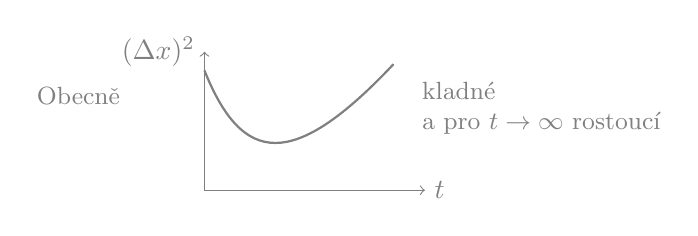
\begin{tikzpicture}[gray,scale=0.8]
  \node at (-2,1.5) {\small Obecně};
  \draw[->] (0,0) -- (0,2.2) node[left] {$(\Delta x)^2$};
  \draw[->] (0,0) -- (3.5,0) node[right] {$t$};
  \draw[thick] (0,1.9) .. controls (0.6,0.4) and (1.4,0.3) .. (3,2);
  \node[right,align=left,font=\small] at (3.3,1.3) {kladné\\a pro $t\to\infty$ rostoucí};
\end{tikzpicture}
\end{center}
DK: $\langle xp + px\rangle$ je $0$, dokud je $\psi(x)$ nebo $\psi(p)$ reálné \\
\quad např.\ $\psi(x)$ \dots \quad
$\langle xp\rangle = \braket{\phi_x}{\phi_p} = i\cdot$reál.\ číslo $= -i\hbar\int\psi(x)\cdot x\,\psi'(x)$ \\
\quad $\ket{\phi_x} \equiv x\ket{\psi}$ \quad\ \
$\langle px\rangle = \braket{\phi_p}{\phi_x} = -i\cdot$stejné číslo $= \big(\braket{\phi_x}{\phi_p}\big)^*$ \\
\quad $\ket{\phi_p} \equiv p\ket{\psi}$ \quad pokud je $p_0\neq 0$ i $x_0\neq 0$, pak $\psi(x)$ i $\psi(p)$ jsou komplexní, \\
\hspace*{2cm} ale $\langle xp+px\rangle$ bylo $0$ s \ $\psi(x) = \frac{1}{\sqrt{\cdots}}e^{-\frac{(x)^2}{(2\Delta x)^2}}e^{\frac{i}{\hbar}p_0x}$ \\
$\to$ záměna $x\to x - x_0$ \quad $\langle(x-x_0)p + p(x-x_0)\rangle = 0 = \langle xp+px\rangle - 2x_0p_0$
\end{priklad}

%----------------------------------------------------------------------
\strana{QM-T-7}
\begin{priklad}[PŘ: Lineární harmonický oscilátor v Heisenberg.\ repr.]
\[
  \left.\begin{aligned}
    \dot x_H &= \frac{1}{i\hbar}[x_H,H] = \frac{p_H}{m} \\
    \dot p_H &= \frac{1}{i\hbar}[p_H,H] = -m\omega^2x_H = -kx_H
  \end{aligned}\right\}\ \text{jako klas.\ rovnice, ale pro operátory}
\]
\[
  \text{\underline{důsl}:}\quad
  \left.\begin{aligned}
    \frac{\dd}{\dd t}\langle x\rangle &= \frac1m\langle p\rangle \\
    \frac{\dd}{\dd t}\langle p\rangle &= -k\langle x\rangle
  \end{aligned}\right\}\
  \begin{minipage}{0.45\textwidth}
  střední hodnoty splňují stejné rce jako klas, bez ohledu na stav \\ (může být zcela neklasický)
  \end{minipage}
\]
ale \pozor{pozor}: $x,p$ nekompatibilní pozorovatelné $\nearrow$
\end{priklad}

\subsubsection*{Koherentní (kvaziklasické) stavy LHO}
\underline{cíl:}
\begin{itemize}[nosep]
  \item[--] najít kvantový stav $\ket{\psi}$ LHO, který se v limitě $E\gg\hbar\omega$ bude podobat klasické částici.
  \item[--] vedlejší produkt: najdeme vývoj Gauss.\ balíku pro LHO
\end{itemize}
vidíme, že $\langle x\rangle$ a $\langle p\rangle$ automaticky klas.\ pohyb. \\
$\to$ další požadavky: $\Delta x,\Delta p$ malé a $E = H_{\text{klas}}(\langle x\rangle,\langle p\rangle)$; $\Delta E$ malé \\
$\to$ vyjde: důležité jsou vl.\ st.\ $\hat a = (\hat q + i\hat p)/\sqrt2$

v klasické fyzice: \quad $a = a_0e^{-i\omega t}$ \quad \dots\ může zkusit, že Heisenbergova rovnice \\
\hspace*{3cm} $\hookrightarrow\ \equiv\frac{1}{\sqrt2}(q_0 + ip_0)$ \hspace{1.5cm} $\Rightarrow$ \quad $\hat a_H = \hat a_S\cdot e^{-i\omega t}$

vyjdeme z:
\begin{itemize}
  \item \underline{požadavek:} \quad
        $\langle E\rangle \equiv \langle\hbar\omega(\hat N + \tfrac12)\rangle = \hbar\omega\langle a^\dagger a\rangle + \underbrace{\tfrac{\hbar\omega}{2}}_{\substack{\text{zanedb}\\ \text{pro } E\gg\hbar\omega}}
         = \hbar\omega\cdot|a_0|^2 = \frac{\hbar\omega}{2}(p^2 + q^2)$
\end{itemize}
\quad tj.\ současně: \ (1) $\langle a\rangle = a_0 \equiv \frac{1}{\sqrt2}(q_0 + ip_0)$ \\
\quad $E\gg\hbar\omega$ \qquad\quad (2) $\langle a^\dagger a\rangle = |a_0|^2$
\[
  \Rightarrow\ \text{platí jen ve stavu}\quad a\ket{\psi} = a_0\ket{\psi} \overset{\text{def}}{\equiv} \alpha\ket{\psi}
  \quad\to\ \text{def: \kw{koherentní stav}}
\]
\underline{pozn:} základní stav $\ket{0}$ je koh.\ stavem pro $\alpha = 0$, ale semiklasický jen pro $\alpha\gg1$

\noindent\rule{0.7\linewidth}{0.3pt} \\
\underline{DK:} \quad def \ $\ket{v} = a\ket{\psi} - a_0\ket{\psi}$
\[
  \text{pak}\quad 0 \leq \braket{v}{v} = \underbrace{\mel{\psi}{a^\dagger a}{\psi}}_{|a_0|^2} - a_0^*\underbrace{\mel{\psi}{a}{\psi}}_{=a_0}
  - a_0\underbrace{\mel{\psi}{a^\dagger}{\psi}}_{=a_0^*} + |a_0|^2\underbrace{\braket{\psi}{\psi}}_{=1}
\]
\quad tj.\ $0 = \braket{v}{v}$, ale rovnost $\curvearrowleft$ platí jen pro $\ket{v} = 0$ \quad (def.\ skalár.\ souč.\ v LVP) \\
\noindent\rule{0.7\linewidth}{0.3pt}

dále budeme vyšetřovat vlastnosti koh.\ st.\ a ukážeme, že splňuje $\forall$ podmínky hledané na klas.\ lim pro $\alpha\gg1$

\sout{$\bullet$ $\Delta x,\Delta p$ je malé} \ \underline{vyjádření $\ket{\psi}\equiv\ket{\alpha}$ ve stac.\ stavech pro LHO}
\[
  \ket{\alpha} = \sum_n c_n\ket{n} \ \to\ \hat a\ket{\alpha} = \alpha\ket{\alpha} \ \Rightarrow\ c_{n+1} = \frac{\alpha}{\sqrt{n+1}}c_n
\]
tj.\ \quad $\ket{\alpha} = N\sum_n\frac{\alpha^n}{\sqrt{n!}}\ket{n}$ \quad + normování \quad
$\braket{\alpha}{\alpha} = \sum_n\frac{|\alpha|^{2n}}{n!} = e^{|\alpha|^2}$ \quad $\Rightarrow$ \quad $N = e^{-|\alpha|^2/2}$

%----------------------------------------------------------------------
\strana{QM-T-8}
\underline{Měření energie:} \quad $p_n = |c_n|^2 = \dfrac{|\alpha|^{2n}}{n!}e^{-|\alpha|^2}$ \quad $\to$ \kw{Poissonovo rozdělení}

maximum? \quad $p_n = \frac{|\alpha|^2}{n}p_{n-1}$ \quad $\to$ max pro $|\alpha|^2\simeq n$
\[
  \langle E\rangle \equiv \langle H\rangle = \sum p_n\underbrace{E_n}_{\hbar\omega(n+\frac12)} = \text{(dá se spočíst analyt.)}
  \underset{\text{ale níže}}{=} \hbar\omega\big(\langle a^\dagger a\rangle + \tfrac12\big) = \hbar\omega\big(|\alpha|^2 + \tfrac12\big)
\]
rozptyl $\Delta E$? (variance)
\begin{align*}
  \langle H^2\rangle &= \hbar^2\omega^2\mel{\alpha}{(a^\dagger a + \tfrac12)^2}{\alpha}
   = \hbar^2\omega^2\bra{\alpha}\big(a^\dagger\underbrace{aa^\dagger}_{=a^\dagger a + [a,a^\dagger]}a + a^\dagger a + \tfrac14\big)\ket{\alpha} \\
  &= \hbar^2\omega^2\big(|\alpha|^4 + 2|\alpha|^2 + \tfrac14\big)
\end{align*}
\[
  \to\quad \Delta E^2 = \langle H^2\rangle - \langle H\rangle^2 = \hbar^2\omega^2|\alpha|^2
  \quad\to\quad \vzorec{\frac{\Delta E}{\langle E\rangle} \simeq \frac{1}{|\alpha|} \ll 1}\ \text{ v lim } n\to\infty
\]

\underline{hodnoty $\Delta x,\Delta p$?} \quad \dots\ automaticky \quad
$\left.\begin{aligned}
  \langle x\rangle &= x_0\sqrt2\cdot\operatorname{Re}\alpha = x_c \\
  \langle p\rangle &= p_0\sqrt2\cdot\operatorname{Im}\alpha = p_c
\end{aligned}\right\}$ \dots\ klasické \\
\hspace*{9cm} \pozn{$x_0 = \sqrt{\frac{\hbar}{m\omega}}$, \ $p_0 = \frac{\hbar}{x_0}$}
\[
  \left.\begin{aligned}
    \langle x^2\rangle_\alpha &= \frac{x_0^2}{2}\big[(\alpha+\alpha^*)^2 + 1\big] \\
    \langle p^2\rangle_\alpha &= \frac{p_0^2}{2}\big[1 - (\alpha-\alpha^*)^2\big]
  \end{aligned}\right\}
  \Rightarrow\
  \begin{aligned}
    \Delta x &= \frac{x_0}{\sqrt2} \\
    \Delta p &= \frac{p_0}{\sqrt2}
  \end{aligned}
  \ \Rightarrow\ \vzorec{\Delta x\cdot\Delta p = \frac{\hbar}{2}}
\]
\hfill \dots\ \underline{minimalizuje neurč.!}

\underline{zápis $\ket{\alpha}$ v $x$-reprezentaci:}
\[
  \text{platí:}\quad \psi_\alpha(x) = e^{i\theta_\alpha}\sqrt[4]{\frac{1}{2\pi(\Delta x)^2}}\cdot
  \exp\Big\{-\Big(\frac{x - \langle x\rangle}{2\Delta x}\Big)^2 + \frac{i}{\hbar}\langle p\rangle x\Big\}
\]
\dots\ tj.\ \kw{minimalizující Gauss balík}

\pozn{
DK: 1) všimněte si, že zákl.\ stav $\braket{x}{0} = \phi_0\big(\frac{x}{x_0}\big)\frac{1}{\sqrt{x_0}}$, \ $\phi_0 = \frac{1}{\sqrt[4]{\pi}}e^{-\frac12q^2}$ \\
\quad splňuje $\uparrow$ s $\Delta x = \frac{x_0}{\sqrt2}$ a $\langle x\rangle = 0$ \\[2pt]
2) Najdeme unit.\ operátor $D(\alpha)$: $\ket{0}\to\ket{\alpha}$
\[
  \ket{\alpha} = e^{-|\alpha|^2/2}\sum_n\frac{\alpha^n}{\sqrt{n!}}\ket{n} = e^{-|\alpha|^2/2}\sum_n\frac{(\alpha a^\dagger)^n}{n!}\ket{0} = e^{-|\alpha|^2/2}e^{\alpha a^\dagger}\ket{0}
\]
\dots\ není unit., ale \ $D(\alpha) = e^{\alpha a^\dagger - \alpha^*a} = e^{-|\alpha|^2/2}e^{\alpha a^\dagger}e^{-\alpha^*a}$ \\
je unitární, a $e^{-\alpha^*a}\ket{0} = \ket{0}$ \hfill $\hookrightarrow$ užití $e^Ae^B = e^{A+B}\cdot e^{\frac12[A,B]}$ \\[2pt]
tj.\ $\psi_\alpha(x) = \mel{x}{D(\alpha)}{0} =$
\[
  D(\alpha) = \exp\Big\{\underbrace{\tfrac{\alpha-\alpha^*}{\sqrt2}}_{ip_c}\hat q - i\underbrace{\tfrac{\alpha+\alpha^*}{\sqrt2}}_{q_c}\hat p\Big\}
  = \exp\{ip_c\hat q - iq_c\hat p\} = e^{ip_c\hat q}e^{-iq_c\hat p}
  \underbrace{e^{\frac{\alpha^{*2}-\alpha^2}{4}}}_{e^{-\frac12[\hat q,\hat p]p_cq_c} = e^{\frac{i}{2}p_cq_c} = e^{i\theta_\alpha}}
\]
\[
  \text{tj.}\quad \psi_\alpha(x) = \bra{x}e^{ip_c\hat q}e^{-iq_c\hat p}\ket{0}
  = e^{\frac{i}{\hbar}\langle p\rangle\cdot x}\underbrace{\bra{x}e^{-\frac{i}{\hbar}\langle x\rangle\hat p}\ket{0}}_{\substack{\text{posunutí o }\langle x\rangle\\ \to\ \braket{x}{0}|_{x = x-\langle x\rangle}}}
  \qquad \hat q = \frac{\hat x}{x_0} = \frac{p_0}{\hbar}\hat x
\]
$\Rightarrow$ c.b.d. \qquad pozn: dá se alternativně DK z vyjádření $\ket{\alpha} = \sum_n c_n\ket{n}$ v $x$-repr.\ pomocí Hermite + rozgenerující fce $H_n$
}

%----------------------------------------------------------------------
\strana{QM-T-9}
\underline{časový vývoj?}
\[
  \text{platí}\quad \ket{\alpha(t)} = \sum_n c_ne^{-\frac{i}{\hbar}E_nt}\ket{n} = e^{-i\omega t/2}\sum_n\frac{(\alpha e^{-i\omega t})^n}{\sqrt{n!}}\ket{n}\cdot e^{-|\alpha|^2/2}
\]
\[
  \text{tj.}\quad \vzorec{\ket{\alpha(t)} = e^{-i\omega t/2}\ket{\alpha = \alpha_0e^{-i\omega t}}}
\]
$\Rightarrow$ zůstává koher.\ stavem s $\alpha$ měnícím se podle klas.\ fyziky \\
$\Rightarrow$ Gaussův balík zůstává, jen se posouvá $\langle x\rangle,\langle p\rangle$ \dots\ jako klas.\ fyz. \\
\quad navíc zůstává $\Delta x\Delta p = \frac{\hbar}{2}$ a $\langle E\rangle$ se samozřejmě zachovává

%----------------------------------------------------------------------
\strana{QM-T-10}
\subsection{Evoluční operátor pro $H(t)$ \ {\normalfont\small -- až nakonec kapitoly}}
\pozn{v originále stránka označená QM-T-\sout{8} 10}
\[
  \ket{\psi(t)} = U(t,t_0)\ket{\psi(t_0)}
\]
(SRt) $\to$ \quad $i\hbar\pdv{t}U(t,t_0) = H(t)U(t,t_0)$ \quad \dots\ s poč.\ podm.\ $U(t_0,t_0) = I$

integrací: \quad $U(t,t_0) = I + \dfrac{1}{i\hbar}\displaystyle\int_{t_0}^{t}H(t_1)U(t_1,t_0)\,\dd t_1 = \mathcal{F}[U]$

\quad iterování \quad $U^{(0)} = I$: \quad $U^{(n+1)} = \mathcal{F}[U^{(n)}]$
\begin{align*}
  \to\ U(t,t_0) = I &+ \frac{1}{i\hbar}\int_{t_0}^{t}H(t_1)\,\dd t_1 + \Big(\frac{1}{i\hbar}\Big)^2\int_{t_0}^{t}\int_{t_0}^{t_1}H(t_1)H(t_2)\,\dd t_2\dd t_1 + \dots \\
  \text{($*$) \kw{Dysonova řada}} \quad &+ \Big(\frac{1}{i\hbar}\Big)^n\int_{t_0}^{t}\int_{t_0}^{t_1}\!\!\cdots\int_{t_0}^{t_{n-1}}H(t_1)H(t_2)\cdots H(t_n)\,\dd t_n\cdots\dd t_2\dd t_1 + \dots
\end{align*}

\begin{itemize}
  \item dá se zkonstruovat $\{H(t)\}$: \quad $[H(t_1),H(t_2)] = 0$ \quad \dots\ ne moc častý příp.
\end{itemize}
\begin{minipage}{0.7\textwidth}
pak
\begin{align*}
 \int_{t_0}^{t}\int_{t_0}^{t_1}H(t_1)H(t_2)\,\dd t_2\dd t_1
 &= \frac12\Big[\int_{t_0}^{t}\int_{t_0}^{t}H(t_1)H(t_2)\,\dd t_1\dd t_2\Big] \\
 &= \frac12\Big[\int_{t_0}^{t}H(t')\,\dd t'\Big]^2
\end{align*}
\end{minipage}\hfill
\begin{minipage}{0.25\textwidth}
\begin{tikzpicture}[gray,scale=0.9]
  \draw[->] (0,0) -- (0,2) node[left] {$t_2$};
  \draw[->] (0,0) -- (2.2,0) node[below] {$t_1$};
  \fill[pattern=north east lines,pattern color=gray] (0,0) -- (1.7,1.7) -- (1.7,0) -- cycle;
  \draw[dashed] (0,0) -- (1.8,1.8);
  \draw[dotted] (1.7,0) -- (1.7,1.7);
\end{tikzpicture}
\end{minipage}

podob. \quad
$\displaystyle\int_{t_0}^{t}\int_{t_0}^{t_1}\!\!\cdots\int_{t_0}^{t_{n-1}}H(t_1)\cdots H(t_n)\,\dd t_n\cdots\dd t_1 = \frac{1}{n!}\Big[\int_{t_0}^{t}H(t')\,\dd t'\Big]^n$
\[
  \to\quad U(t,t_0) = \exp\Big\{-\frac{i}{\hbar}\int_{t_0}^{t}H(t')\,\dd t'\Big\}
\]

\begin{itemize}
  \item \underline{obecně:} zavedeme \kw{čas.\ uspořádání} \quad $T\big(H(t_i)H(t_j)\big) = H(t_<)H(t_>)$ \\
        \hspace*{6cm} $t_< \equiv \min(t_1,t_2)$, \ $t_> = \max(t_1,t_2)$
\end{itemize}
pak \quad $T\big([H(t_1),H(t_2)]\big) = 0$, a tedy
\begin{align*}
  \int_{t_0}^{t}\cdots\int_{t_0}^{t_{n-1}}H(t_1)\cdots H(t_n)\,\dd t_n\cdots\dd t_1
  &= \frac{1}{n!}\int_{t_0}^{t}\dd t_1\cdots\int_{t_0}^{t}\dd t_n\,T\big(H(t_1)\cdots H(t_n)\big) \\
  &= \frac{1}{n!}T\Big(\Big[\int_{t_0}^{t}\dd t'\,H(t')\Big]^n\Big)
\end{align*}
\[
  \to\quad \vzorec{U(t,t_0) = T\exp\Big\{-\frac{i}{\hbar}\int_{t_0}^{t}H(t')\,\dd t'\Big\}}
\]
\dots\ vypadá zběsile, ale s úspěchem se používá \\
\quad $\to$ výhodné pro poruch.\ rozvoje v mocninách operátorů
